\begin{dfn}[Angle]
Let \(P\) be an ordered geometry and \(x\), \(o\), and \(y\) distinct points.
Then the set \[ \ANGLE{x}{o}{y} = \RAY{o}{x} \cup \RAY{o}{y} \] is called the \emph{angle}\index{angle} with \emph{vertex} \(o\) and \emph{sides} \(\RAY{o}{x}\) and \(\RAY{o}{y}\).
If \(\BETWEEN{x}{o}{y}\), then we say the angle is \emph{straight}\index{angle!straight}, and if \(\BETWEEN{o}{x}{y}\) or \(\BETWEEN{o}{y}{x}\), then we say the angle is \emph{flat}\index{angle!flat}.
\begin{itemize}
\item Suppose \(x\), \(o\), and \(y\) are not collinear.
In this case, since \(P\) is an ordered geometry, the lines \(\LINE{o}{x}\) and \(\LINE{o}{y}\) divide \(P\) into half-planes.
Let \(H_1\) be the \(y\) half-plane of \(\LINE{o}{x}\), and let \(K_1\) be the \(x\) half-plane of \(\LINE{o}{y}\).
We define the \emph{interior} of \(\ANGLE{x}{o}{y}\) to be the set \[ \INTANGLE{x}{o}{y} = H_1 \cap K_1. \]
If \(x\), \(y\), and \(o\) are collinear, then the interior of \(\ANGLE{x}{o}{y}\) is not defined.
\end{itemize}
\end{dfn}

\begin{dfn}[Angle Pairs]
Suppose \(x\), \(y\), \(z\), \(w\), and \(o\) are distinct points in an ordered geometry.
\begin{itemize}
\item \(\ANGLE{x}{o}{y}\) and \(\ANGLE{y}{o}{z}\) are called an \emph{adjacent pair}\index{angle!adjacent pair}.
\item \(\ANGLE{x}{o}{y}\) and \(\ANGLE{y}{o}{z}\) are called a \emph{linear pair}\index{angle!linear pair} if \(\BETWEEN{x}{o}{z}\).
\item \(\ANGLE{x}{o}{y}\) and \(\ANGLE{z}{o}{w}\) are called a \emph{vertical pair}\index{angle!vertical pair} if \(\BETWEEN{x}{o}{z}\) and \(\BETWEEN{y}{o}{w}\).
\end{itemize}
\end{dfn}

\begin{thm}[Crossbar Theorem]
Suppose \(O\), \(A\), and \(B\) are noncollinear points in an ordered geometry, and that \(C \in \INTANGLE{A}{O}{B}\). Then \(\RAY{O}{C}\) cuts \(\SEGMENT{A}{B}\) at a unique point \(D\).
\end{thm}

\begin{center}
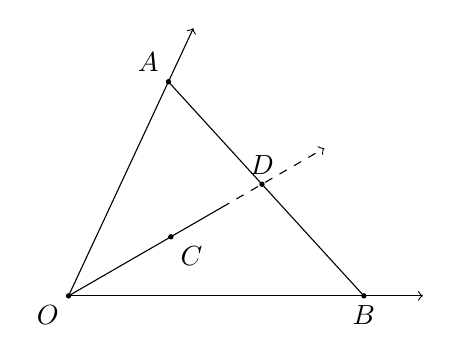
\begin{tikzpicture}[scale=1.5]
  \coordinate [label=below left:\(O\)] (O)   at (0  : 0);
  \coordinate [label=above left:\(A\)] (A)   at (65 : 2);
  \coordinate (A')  at (65 : 2.5);
  \coordinate [label=below:\(B\)]      (B)   at (0  : 2.5);
  \coordinate (B')  at (0  : 3);
  \coordinate (C)   at (30 : 1);
  \coordinate (C')  at (30 : 1.5);
  \coordinate (C'') at (30 : 2.5);

  \coordinate [label=above:\(D\)]      (D)   at (intersection of A--B and O--C'');

  \draw [->] (O) -- (A');
  \draw [->] (O) -- (B');

  \draw [fill] (O) circle [radius=0.5pt];
  \draw [fill] (A) circle [radius=0.5pt];
  \draw [fill] (B) circle [radius=0.5pt];

  \draw (O) -- (C');
  \draw [dashed, ->] (C') -- (C'');

  \draw [fill] (C) circle [radius=0.5pt];
  \node [below right] at (C) {\(C\)};

  \draw (A) -- (B);

  \draw [fill] (D) circle [radius=0.5pt];
\end{tikzpicture}
\end{center}

\begin{proof}
By the Interpolation property, there is a point \(P\) on \(\LINE{O}{A}\) such that \(\BETWEEN{P}{O}{A}\). Note that \(A\) and \(P\) are on opposite sides of \(\LINE{O}{B}\), so that \(P\) and \(C\) are on opposite sides of \(\LINE{O}{B}\). (Since \(A\) and \(C\) are on the same side of \(\LINE{O}{B}\) by definition.) Consider now the triangle \(\TRIANGLE{P}{A}{B}\). Note that the line \(\LINE{O}{C}\) does not contain \(A\), \(B\), or \(P\), since \(C\) is not on \(\LINE{O}{A}\) or \(\LINE{O}{B}\) by hypothesis. Moreover, \(\LINE{O}{C}\) cuts \(\SEGMENT{P}{A}\) at \(O\). By Pasch's Axiom, \(\LINE{O}{C}\) must also cut either \(\SEGMENT{P}{B}\) or \(\SEGMENT{A}{B}\).

Suppose \(\LINE{O}{C}\) cuts \(\SEGMENT{P}{B}\) at a (necessarily unique) point \(Q\). Note that \(\LINE{O}{C} = \LINE{Q}{C}\). Now \(P\) and \(Q\) are on the same side of \(\LINE{O}{B}\), so that \(Q\) and \(C\) are on \emph{opposite} sides of \(\LINE{O}{B}\). Thus, there is a unique point \(R\) on \(\LINE{O}{B}\) such that \(\BETWEEN{Q}{R}{C}\). In particular, \(R \in \LINE{O}{C}\). Now we have \(O,R \in \LINE{O}{C}\) and \(O, R \in \LINE{O}{B}\), so that \(\LINE{O}{C} = \LINE{O}{B}\), a contradiction.

Hence \(\LINE{O}{C}\) must cut \(\SEGMENT{A}{B}\) at a unique point; say \(D\). Now \(D\) and \(A\) are on the same side of \(\LINE{O}{B}\), and so \(C\) and \(D\) are on the same side of \(\LINE{O}{B}\); in particular, we cannot have \(\BETWEEN{D}{O}{C}\). So in fact \(\RAY{O}{C}\) cuts \(\SEGMENT{A}{B}\) at a unique point.
\end{proof}

